 % -*- root: ../medieninformatik-arbeit.tex -*-
\documentclass[../medieninformatik-arbeit.tex]{subfiles}
\begin{document}
	

\section{Related Work}
\label{ch:related}
In this chapter projects related to product configurators and activity
sculptures will be presented. Each work presents a unique solution to the addressed problem, 
the approach each author took will be discussed and the adaptation of useful knowledge to this
work will be explored. To conclude the chapter an overview of available vendor
API for data import will be presented. 

\subsection{Web-based Interactive Product Visualization}
This work has a particular interest in product configurators that make use of 3D
computer graphics to visualize the product. The majority of modern web
configurators are image based and make use of well designed backgrounds to place the
product in well perceived environment. For example the UNU electric scooter
configurator puts the scooter on a street background that
changes as the user moves to the next step of the configuration (fig.\ref{fig:unu-config}). 
Other systems may opt for a more minimalistic look, and will try to isolate the
product and place it in a white background as seen on
figure \ref{fig:timbuk2-config}. 
Although this might work for some products the user still misses some of the benefits of
interacting with a spatial representation the products\cite{vande2009analyzing}.
One of the main challenges of developing  configurator systems is the modeling
of the relation between the product configuration and its visual representation
and the correct rendering of the visual representation in real
time\cite{feliceinteractive}. The advantage of a 3D visualization system
over an image based one, is that the different configurations can be generated on
the fly instead of using complex logic systems to retrieve the correct image
combination from an image database. On the following section, three product
configurators will be presented that use novel 3D visualization technologies to
offer users a robust interactive tools for designing unique products.

\begin{figure}[h]
\captionsetup{width=0.4\textwidth}
\centering
\begin{minipage}{.45\textwidth}
\centering
  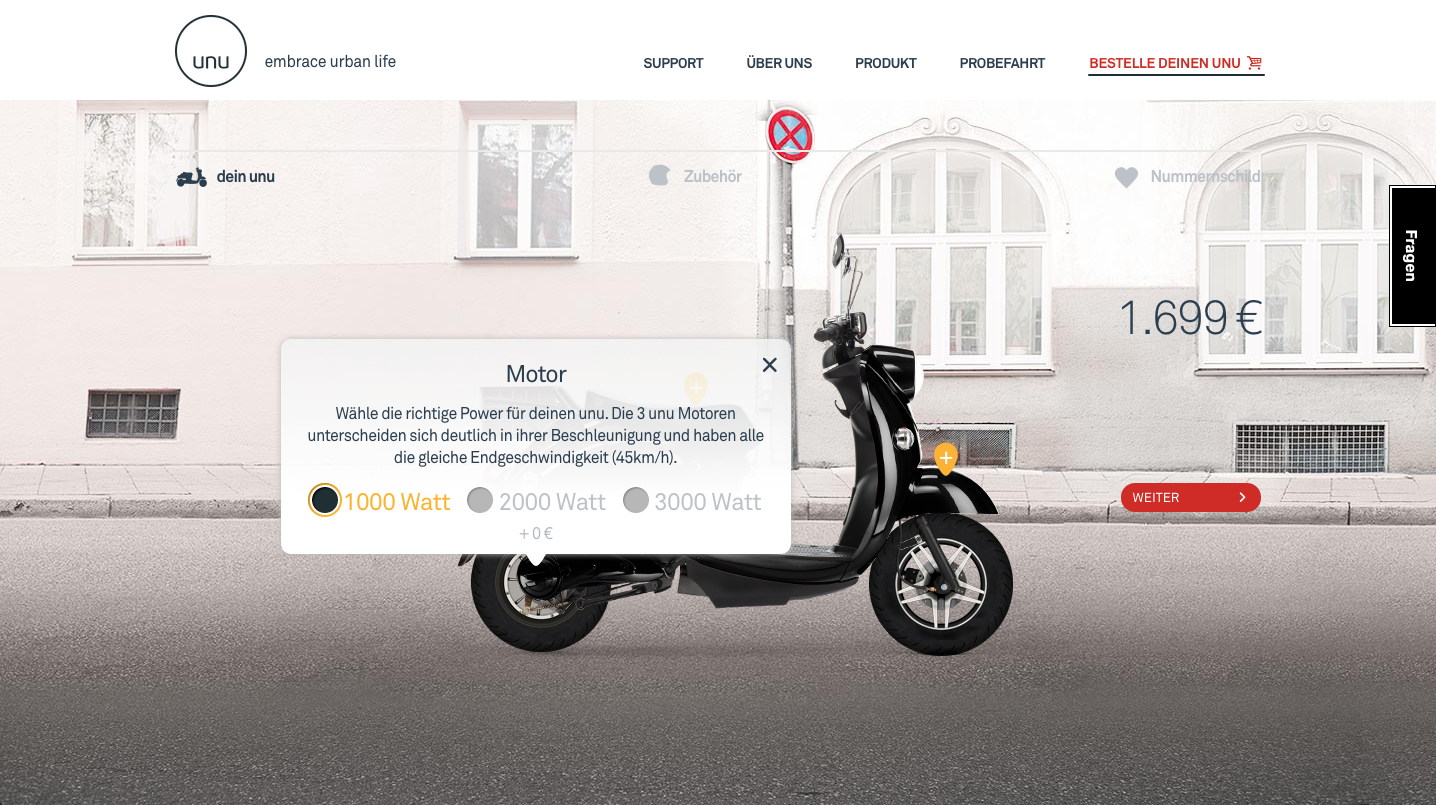
\includegraphics[width=\linewidth]{RelatedWork/img/unu-config}
  \caption{\protect UNU electric scooter web configurator\cite{unu:2015:Online}}
\label{fig:unu-config}
\end{minipage}
\begin{minipage}{.45\textwidth}
\centering
  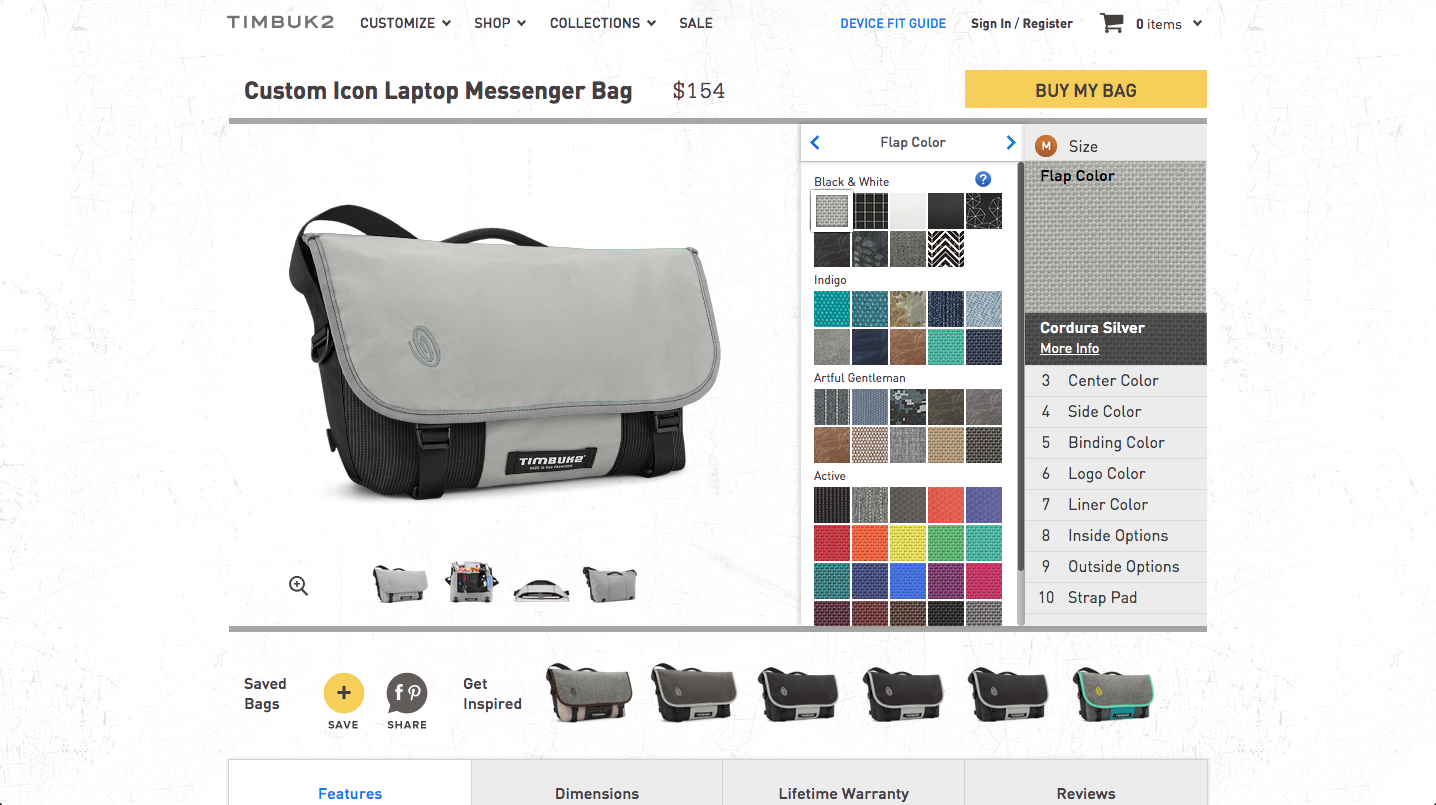
\includegraphics[width=\linewidth]{RelatedWork/img/timbuk2-config}
  \caption{\protect Timbuk2 bag web configurator\cite{timbuk2:2015:Online}}
\label{fig:timbuk2-config}
\end{minipage}
\end{figure}

\subsubsection{Gates 3D Configurator}
As part of an action-research project from Living
Lab\cite{livinglabs:2015:Online} Rolland et al.\cite{rolland2012commerce}
developed a gate configurator for the French company Groupe Maine's gates. The
objective of the authors was to showcase the possibilities of 3D Web
technologies in e-commerce applications. The developed tool was build with the
Unitiy3D\cite{unity3d:2015:Online} game engine, a flexible tool principally
build for game development but it has proved to be also useful for architectural
visualization and graphic intense web applications. After a user has logged in
to the configurator, the platform allows customers to select from a variety of
gate styles visualized as 3D models placed on the right side controls (see fig.\ref{fig:gates-config}). The user has also the option of setting the environment in which the gate is being placed (left side controls). This can happen by either selecting a predefined environment of by uploading a picture of the user's home or place where the gate shall be installed later. Customers can position the gates in the uploaded photograph by operating dedicated slider controls. The main advantage of allowing customers to upload their own images is that this allows them to have a better idea of how the selected gates will look in the final environment making them feel more comfortable about their decision. The authors state that they preferred the superimposition of a custom image rather than letting the user customize the environment with threes or buildings to make it look as close as possible because of the possible frame rate drop produced of handling many models and generating and because it is quite rare that somebody has a 3D model of his home. 

One of the main aspects of the gates configurator in respect to the research purposes the authors had, was that of developing a tool that improved the visualization of products with the end of encouraging the purchasing of the product in an on-line medium. To validate the design ideas behind the gate configurator and analyze the impact it had on customers, the authors performed an empirical evaluation. The results of the 27 evaluated participants showed that the manipulation of objects in 3D space seem naturally and was also confirmed to be important to the participants to have this option. This shows that having a realistic view of the product improves the chances of sale.

\begin{figure}[hb]
\begin{center}
  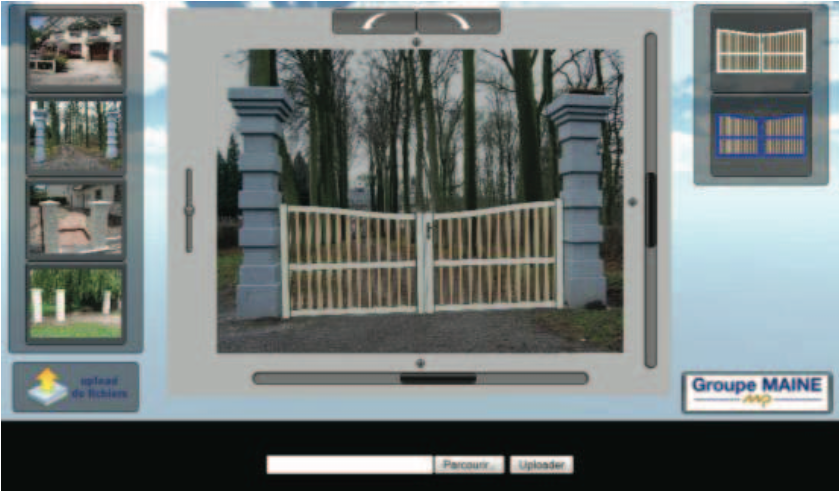
\includegraphics[width=0.7\textwidth]{RelatedWork/img/gates-config}
  \caption{Groupe Maine's configurator\cite{rolland2012commerce} }
\label{fig:gates-config}
\end{center}
\end{figure}

The gates configurator is a great example of how companies can make use of 3D visualization technologies to present their product to customers in a more convincing way. The authors of made a great choice of working with the Unity3D game engine as it allows them to port to other platforms as well, in this way developed software tools could be very easily ported to other mobile platforms like tablets or smartphones with bigger screens without the need of starting from scratch. This technology also offers desktop like frame rate performance in the web. The configurator has not many configuration possibilities which makes it easier for customers to understand but it excels at providing different visualization environments which in this case takes advantage of navigating in 3D space. One key statement of the authors was that tools like the configurator promote customer's participation in the developing of products. It was a shame there is no actual configurator in the Groupe Main's webpage for testing and it is unknown if the configurator was ever implemented in their website. The authors of the gates configurate see a great potential of 3D visualization technologies in fields such as e-learning, simulation and education.

\subsubsection{The MakerVis Fabrication Tool}
The MakerVis fabrication software is, in the words of its creators: \textit{``a prototype tool that integrates the entire process of creating physical visualizations, from data filtering to physical fabrication''}\cite{swaminathan2014supporting}. If somebody attempts to visualize their information they will have to use a wide range of tools to achieve this. This is cumbersome and impractical as it requires a great amount of effort and in general it is a very conflict prone way of working with data. This motivated Swaminathan et. al to develop MakerVis as an attempt to offer a platform that unifies the needed tools to extract data, filter it and visualize it. Although the focus of the MakerVis is not the implementation of a complex tool but more the exploration of the different challenges encountered in the process of visualization.

The work-flow provided by MakerVis is composed of six steps all displayed in the user interface seen on figure \ref{fig:makervis-config}. First users need to upload a CSV file containing the data to visualize. After that users can select between several visualization styles. Once a visualization is selected the data the user can begin mapping the data to the visualization by selecting data variables. Further on users can manipulate the visualization's geometry through an array of sliders and controls. In order to setup fabrication parameters and selecting the machine users can make use of the lower right section where the visualization is deconstructed layer by layer. Finally the STL file of the model can be exported for fabrication. A helpful functionality the authors implemented was the specification of printing materials through a JSON file.  It is worth mentioning that MakerVis does not provide true 3D visualizations. The produced designs are indeed physical objects but the final result is a pseudo 3D visualization. In order to achieve this the authors use principally 2D fabrication methods employing laser cutting and CNC machines, only basic 3D printing support is provided. The visualizations users can choose from are more directed to traditional charts and bar graphs and not so much geared towards more artistic representations. Due to the modular engineering of tool, the visualizations can be expanded. The available tools for data manipulation is also limited and advanced manipulation should be better performed in an external tool. MakerVis was build with modern web technologies based on the JavaScript programming language like Node.js\cite{joyent2015node}, Three.js\cite{cabello2010three}, D3.js\cite{bostock2015d3js} and jQuery\cite{jqf2015jquery}. As some of this technologies were also used in the Activity Sculpture Configurator they will be explained in depth in Chapter \ref{ch:configurator}. 

Although the authors conducted a relative small user study, the results provided valuable information about what areas can be further improved. The user study showed that users wanted more detailed control about the decorative aspects of visualization. Providing tools for personalize text labels and scales increases would allow users to further customize their visualization. Another challenge encountered was that of material representation. It was difficult for users to decide on which materials to use and expressed the desire to physically interact with the available materials. Also the correct scale representation of the object was estimated wrongly by most users. The need of the ability to save and load visualizations was also expressed to be needed. This findings might sound as failures but they only make clear the limitations of the screen as a medium to transmit haptic properties of materials and that unifying every tool needed for data visualization in a tool is an immense challenge.

\begin{figure}[h]
\begin{center}
  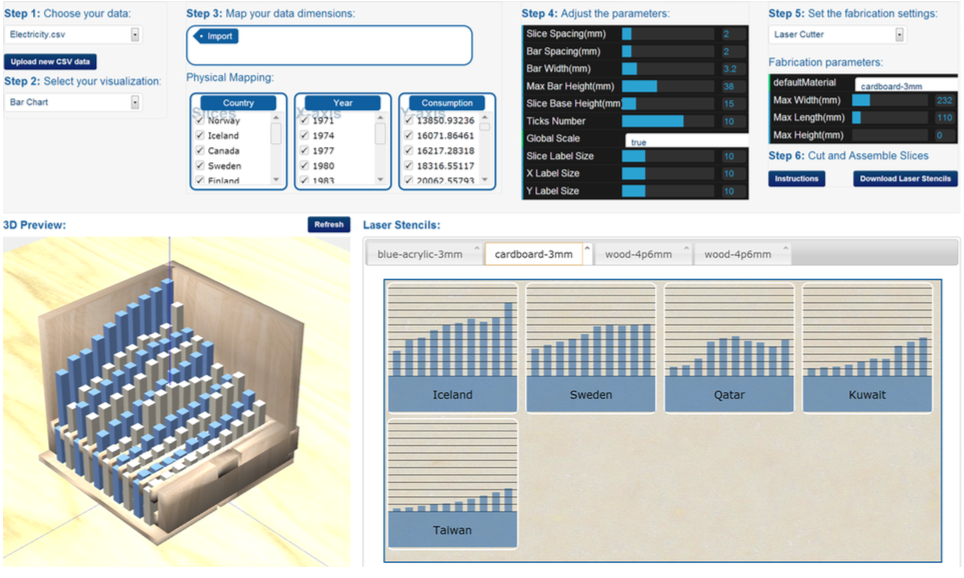
\includegraphics[width=0.7\textwidth]{RelatedWork/img/MakerVis}
  \caption{The MakerVis fabrication tool\cite{swaminathan2014supporting} }
\label{fig:makervis-config}
\end{center}
\end{figure}

The MakerVis fabrication tool approximates closely the aim of the work discussed in this thesis. This work shares the same mission of building a tool were the whole process of visualizing a 3D object is contained. The MakerVis focuses more on data manipulation and fabrication as it basically dedicates two thirds of the whole screen to data filtering and fabrication parameters. None the less the interaction concepts and design layout served as a reference point for the activity sculpture configurator. 

\subsubsection{Twikit}


\begin{figure}[h]
\captionsetup{width=0.4\textwidth}
\centering
\begin{minipage}{.45\textwidth}
\centering
  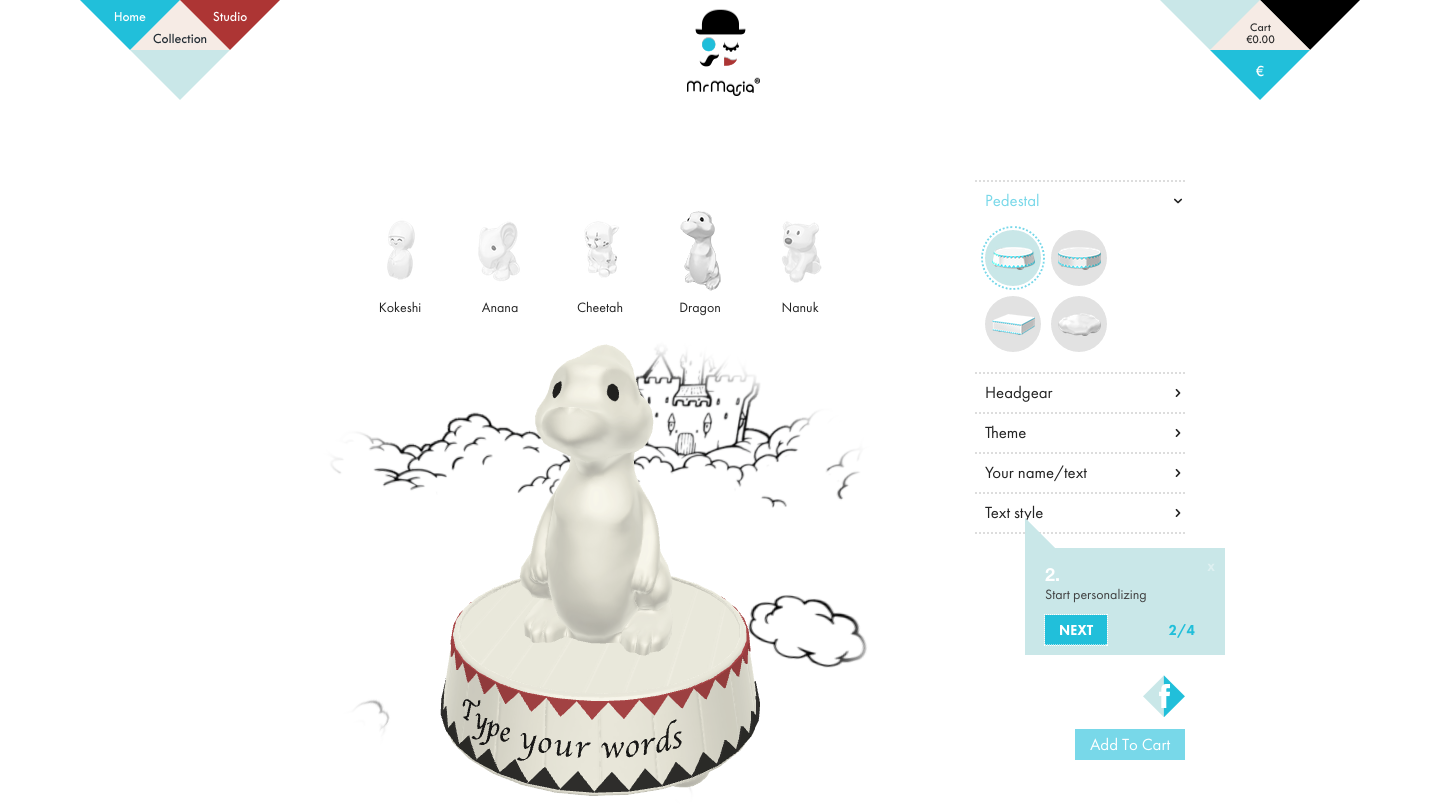
\includegraphics[width=\linewidth]{RelatedWork/img/mrmaria-config}
  \caption{\protect Twikit powered MrMaria Studio lamp web configurator\cite{unu:2015:Online}}
\label{fig:mmaria-config}
\end{minipage}
\begin{minipage}{.45\textwidth}
\centering
  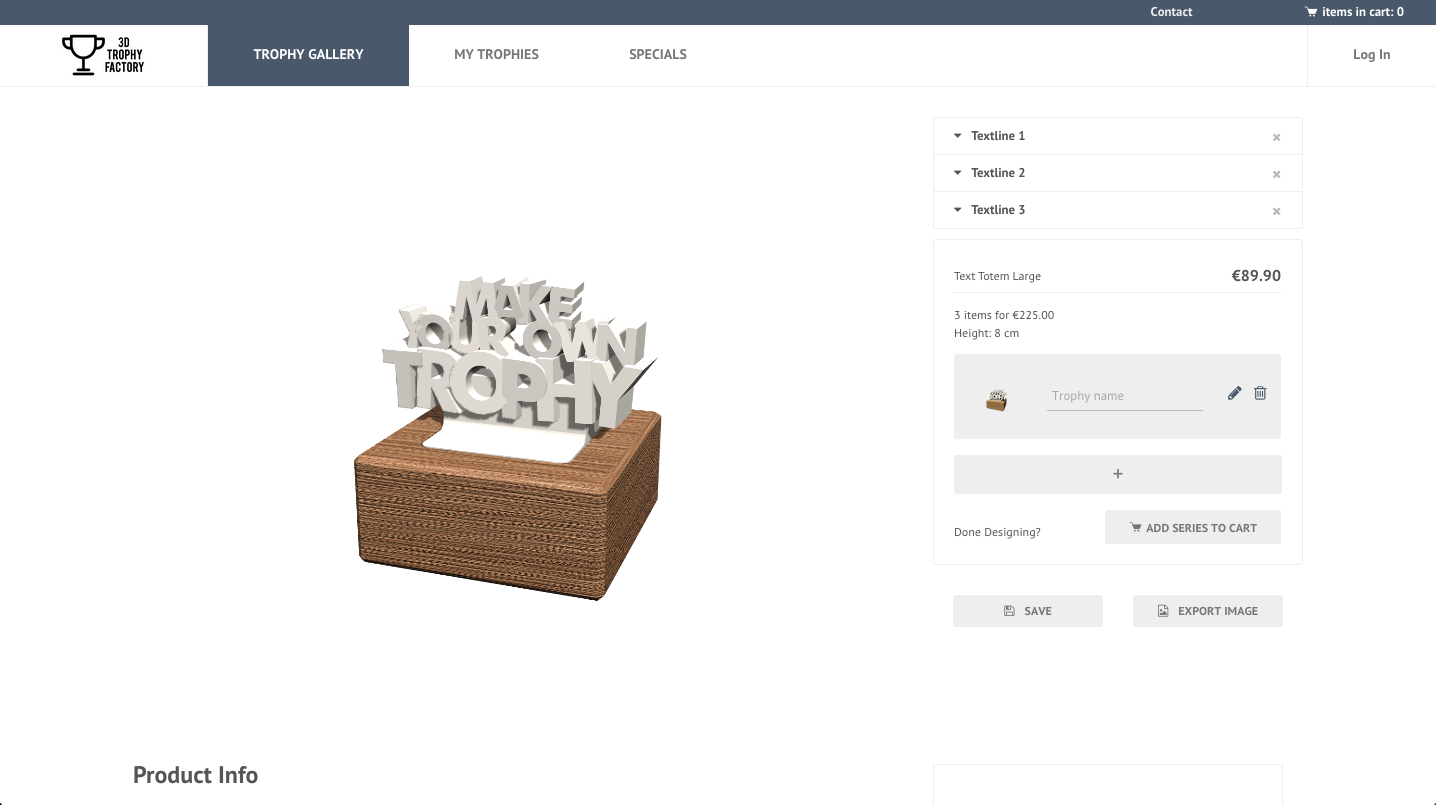
\includegraphics[width=\linewidth]{RelatedWork/img/trophy-config}
  \caption{\protect Twikit powered 3D Trophy Factory web configurator\cite{timbuk2:2015:Online}}
\label{fig:trophy-config}
\end{minipage}
\end{figure}


\subsection{Activity Sculptures}
see \cite{swaminathan2014supporting} for more sources about activity sculptures, good stuff in there!

\subsubsection{Sweet Atoms}

\subsubsection{Mental Fabrications}

\subsection{Activity Data Sources}

\subsubsection{Fitness Tracker APIs}
\end{document}